\documentclass[17pt,a4paper]{extreport}
\usepackage{graphicx}
\usepackage{amsmath}
\usepackage{mathtools}
\usepackage{hyperref}
\usepackage{tocbibind}
\usepackage{wrapfig}
\usepackage{float}
%\usepackage{subcaption}
\hypersetup{
	colorlinks=true,
	urlcolor=red,
	linkcolor=red,
}

\begin{document}
	\chapter[Results and Discussion]{Results and Discussion}
	\section[Process parameters]{Process parameters}
	The tolerance curves for the various equipments have been taken from standard test data published by manufacturers and various testing centres. Some of them are listed in \cite{Voltage
sag analysis case studies}-\cite{A probabilistic method for comprehensive voltage sag
management in power distribution systems}. For devices except contactors, rectangular tolerance curves were employed. 
\paragraph{} The sag data was obtained from Uttarpradesh chemical plant voltage data.
The bus corresponds to IEEE 32-bus system. The results were computed for all buses, but results for bus 1,2,5 are shown in corresponding trip analysis results.
\paragraph{} The various tolerance curve parameters for the equipments PC, PLC, ASD, 5 h.p ac drive and Motor Starter are shown in below table:
\begin{center}
\begin{table}
\begin{tabular}{|c|c|c|c|c|c|}
\hline
	Sl No. & Equipment & $V_{max}$(\%) & $V_{min}$(\%)& $T_{max}$(ms) & $T_{min}$(ms)\\
	\hline
	1 & PC & 63 & 46 & 205 & 40\\ 
	\hline
	2 & PLC & 90 & 30 & 400 & 20\\
	\hline 
	3 & ASD & 71 & 59 & 175 & 15\\
	\hline
	4 & 5 h.p ac drive &80 & 60 & 80 & 30\\
	\hline
	5 & Motor Starter & 60& 40 & 80& 20\\
	\hline

\end{tabular}
\caption{Tolerance curves}
\label{tab:tolerance_r}
\end{table}
\end{center}
\section[Personal Computers]{Personal Computers}
	The personal computer of tolerance parameters given in table were tested against sag data used in 132 KV bus system. The trip probability was calculated for the sag data, and thresholded at 0.5 to illustrate a trip. Accordingly, the following trip data was observed:
	\paragraph{ } Bus 5 had around 3840 sag points. Figure \ref{fig:pc_sag_5} shows the various sag points , where the blue dotted points indicate that no trip will occur, whereas a red starred point indicates a trip will occur.
	\begin{figure}[!h]
		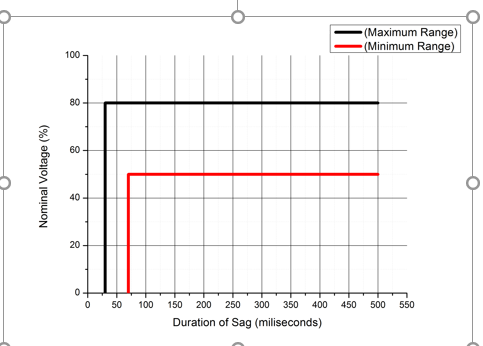
\includegraphics[width=\textwidth]{pc.eps}
		\caption{sag profile for bus 5 with PC}
		\label{fig:pc_sag_5}
	\end{figure}
	The corresponding probability distribution is also indicated by a scatter plot in Figure\ref{fig:scatter_pc_5}.
	\begin{figure}[!h]
	\includegraphics[width=\textwidth]{scatter_pc}
	\caption{ Trip probability for PC in bus 5}
	\label{fig:scatter_pc_5}
\end{figure}	
 The trip data for three buses are given in \ref{tab:PC_res} :
 \begin{center}
 \begin{table}
 \centering
 \caption{Trip data for three buses for PC}
 \begin{tabular}{|c|c|}
 \hline 
 Bus & Number of trips \\ \hline
 1 & 4595 \\ \hline
 2 & 4853 \\ \hline
 5 & 604	\\ \hline
 
 \end{tabular}
 \label{tab:PC_res}
 \end{table}
 
 \end{center}

\newpage \section[PLC]{PLC}
	The PLC was similarly tested, with parameters given in \ref{tab:tolerance_r}, with bus data for buses 5,11,13. The probability was thresholded to 0.5. The following trip data was observed:
	\paragraph{} Figure \ref{fig:plc_sag_5} shows the various sag points , where the blue dotted points indicate that no trip will occur, whereas a red starred point indicates a trip will occur.
	\begin{figure}[!h]
		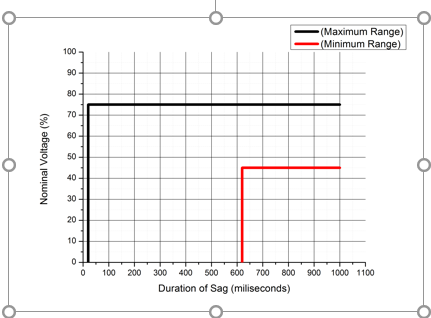
\includegraphics[width = \textwidth]{plc.eps}
		\caption{sag profile for bus 5 with PLC}
		\label{fig:plc_sag_5}
	\end{figure}
	The corresponding probability distribution is also indicated by a scatter plot in Figure\ref{fig:scatter_plc_5}.
	\begin{figure}[h]
	\includegraphics[width = \textwidth]{scatter_plc}
	\caption{Trip probability for PLC in bus 5}
	\label{fig:scatter_plc_5}
\end{figure}

	 The trip data for three buses are given in \ref{tab:PLC_res} :
 \begin{center}
 \begin{table}
 \centering
 \begin{tabular}{|c|c|}
 \hline 
 Bus & Number of trips \\ \hline
 1 & 1567 \\ \hline
 2 &  1727\\ \hline
 5 & 73	\\ \hline
 
 \end{tabular}
 \caption{Trip data for three buses for PLC}
 \label{tab:PLC_res}
 \end{table}
 
 \end{center}
	 \section[ASD]{ASD}
	 The ASD parameters were determined from table \ref{tab:tolerance_r}. The trip probability was similarly calculated for a threshold probability of 0.5. The following trip data was observed: 
	 \paragraph{ } Figure \ref{fig:asd_sag_5} shows the various sag points , where the blue dotted points indicate that no trip will occur, whereas a red starred point indicates a trip will occur.
	\begin{figure}[!h]
		\includegraphics[width = \textwidth]{asd}
		\caption{sag profile for bus 5 with asd}
		\label{fig:asd_sag_5}
	\end{figure}
	The corresponding probability distribution is also indicated by a scatter plot in Figure\ref{fig:scatter_asd_5}.
	\begin{figure}[!h]
	\includegraphics[width = \textwidth]{scatter_asd}
	\caption{Trip probability for asd in bus 5}
	\label{fig:scatter_asd_5}
\end{figure}	
The trip data for three buses are given in \ref{tab:ASD_res} :
 \begin{center}
 \begin{table}
 \centering
 \begin{tabular}{|c|c|}
 \hline 
 Bus & Number of trips \\ \hline
 1 & 5775 \\ \hline
 2 & 5295 \\ \hline
 5 & 730	\\ \hline
 
 \end{tabular}
  \caption{Trip data for three buses for ASD}
 \label{tab:ASD_res}
 \end{table}

 \end{center}

\newpage \section[5hp AC Drive]{5hp AC Drive}
 The 5hp AC Drive parameters were determined from table \ref{tab:tolerance_r}. The trip probability was similarly calculated for a threshold probability of 0.5. The following trip data was observed: 
	 \paragraph{} Figure \ref{fig:5hp_sag_5} shows the various sag points , where the blue dotted points indicate that no trip will occur, whereas a red starred point indicates a trip will occur.
	\begin{figure}[!h]
		\includegraphics[width=\textwidth]{5hp}
		\caption{sag profile for bus 5 with 5hp AC Drive}
		\label{fig:5hp_sag_5}
	\end{figure}
	The corresponding probability distribution is also indicated by a scatter plot in Figure\ref{fig:scatter_5hp_5}.
	\begin{figure}[!h]
	\includegraphics[width = \textwidth]{scatter_5hp}
	\caption{Trip probability for 5hp AC Drive in bus 5}
	\label{fig:scatter_5hp_5}
\end{figure}	
The trip data for three buses are given in \ref{tab:5hp_res} :
 \begin{center}
 \begin{table}
 \centering
 \begin{tabular}{|c|c|}
 \hline 
 Bus & Number of trips \\ \hline
 1 & 5707 \\ \hline
 2 & 5885 \\ \hline
 5 & 1008	\\ \hline
 
 \end{tabular}
  \caption{Trip data for three buses for 5hp AC Drive}
 \label{tab:5hp_res}
 \end{table}

 \end{center}

\section[Motor Starter]{Motor Starter}
 The Motor Starter parameters were determined from table \ref{tab:tolerance_r}. The trip probability was similarly calculated for a threshold probability of 0.5. The following trip data was observed: 
	 \paragraph{} Figure \ref{fig:ms_sag_5} shows the various sag points , where the blue dotted points indicate that no trip will occur, whereas a red starred point indicates a trip will occur.
	\begin{figure}[!h]
		\includegraphics[width=\textwidth]{motor_starter}
		\caption{sag profile for bus 5 with Motor Starter}
		\label{fig:ms_sag_5}
	\end{figure}
	The corresponding probability distribution is also indicated by a scatter plot in Figure\ref{fig:scatter_ms_5}.
	\begin{figure}[!h]
	\includegraphics[width=\textwidth]{scatter_ms}
	\caption{Trip probability for Motor starter in bus 5}
	\label{fig:scatter_ms_5}
\end{figure}	
The trip data for three buses are given in \ref{tab:ms_res} :
 \begin{center}
 \begin{table}
 \centering
 \begin{tabular}{|c|c|}
 \hline 
 Bus & Number of trips \\ \hline
 1 & 5112 \\ \hline
 2 & 5017 \\ \hline
 5 & 672	\\ \hline
 
 \end{tabular}
  \caption{Trip data for three buses for Motor Starter}
 \label{tab:ms_res}
 \end{table}

 \end{center}
 
 \section[Contactor]{Contactor}
 The Contactor parameters were determined from table \ref{tab:tolerance_r}. The trip probability was similarly calculated for a threshold probability of 0.5. The following trip data was observed: 
	 \paragraph{} Figure \ref{fig:con_sag_5} shows the various sag points , where the blue dotted points indicate that no trip will occur, whereas a red starred point indicates a trip will occur.
	\begin{figure}[!h]
		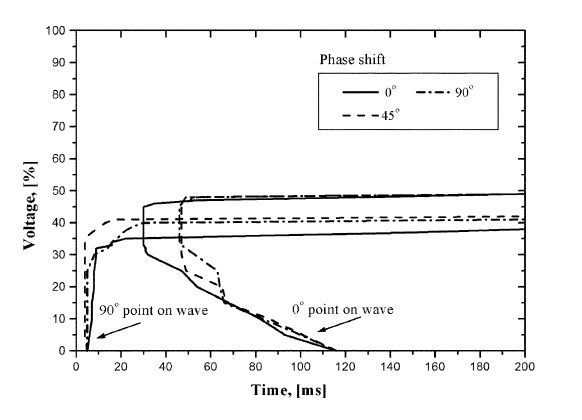
\includegraphics[width=\textwidth]{contactor.eps}
		\caption{sag profile for bus 5 with Contactor}
		\label{fig:con_sag_5}
	\end{figure}
	The corresponding probability distribution is also indicated by a scatter plot in Figure\ref{fig:scatter_con_5}.
	\begin{figure}[!h]
	\includegraphics[width=\textwidth]{contactor_trip_prob}
	\caption{Trip probability for contactor in bus 5}
	\label{fig:scatter_con_5}
\end{figure}	

\newpage \section[Process Trip]{Process Trip} The process trips were calculated for a number of series parallel combinations.Probability distributions for three such will be shown in this part. Six equipments were randomly chosen for forming the processes, as per designations given in table \ref{tab:process_designations}

\begin{table}[!h]
\centering
\caption{Process Designations}
\begin{tabular}{|c|c|c|}
\hline 
Sl no. & Designation & Equipment\\
\hline
1 & A & PC \\
\hline
2 & B & PLC\\
\hline
3 & C & ASD\\
\hline
4 & D & 5hp AC Drive\\
\hline
5 & E & Motor starter\\
\hline
6 & F & PC\\
\hline

\end{tabular}
\label{process_designations}
\end{table}


The individual equipments have the tolerance characteristics as given in \ref{tab:tolerance_r}

Three combinations used are :
\paragraph{All-Series:} In this, the equipments are connected in series, as given in block-diagram:

\begin{figure}[!h]
\centering
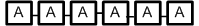
\includegraphics[scale=1]{Drawing6(1).png}
\caption{Block Diagram of All-Series Process}
\end{figure}

The trip probability distribution is given in figure \ref{fig:all-series}


\begin{figure}[!h]
\includegraphics[width=\textwidth]{process_a_series}
\caption{Trip Probability of all-series}
\label{fig:all-series}
\end{figure}
With 3840 sag points, there was 1067 trips observed, which had probability of occurrence of more than 0.5. 

\newpage \paragraph{ All-Parallel:} In this, the equipments are connected in parallel, as given in block-diagram:

\begin{figure}[!h]
\centering
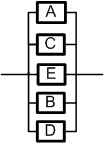
\includegraphics[scale=1]{3.png}
\caption{Block Diagram of Parallel Process}
\end{figure}

The trip probability distribution is given in figure \ref{fig:all-parallel}


\begin{figure}[!h]
\includegraphics[width=\textwidth]{process_a_parallel}
\caption{Trip Probability of all-parallel process}
\label{fig:all-parallel}
\end{figure}
With 3840 sag points, there was 73 trips observed, which had probability of occurrence of more than 0.2. 

\newpage \paragraph{ Series Parallel:} In this, the equipments are connected in parallel sets of two, which are connected in series to form the whole process, as given in block-diagram:

\begin{figure}[!h]
\centering
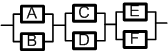
\includegraphics[scale=1]{2.png}
\caption{Block Diagram of Series-Parallel Process}
\end{figure}

The trip probability distribution is given in figure \ref{fig:series-parallel}.


\begin{figure}
\includegraphics[width=\textwidth]{process_series_parallel}
\caption{Trip Probability of series-parallel process}
\label{fig:series-parallel}
\end{figure}
With 3840 sag points, there was 730 trips observed, which had probability of occurrence of more than 0.5. 
\end{document}